\customHeader{1}{Pattern-Exploiting Training}
\label{06_pet}

Few-shot learning is a \gls{ml} technique that aims to train models to generalize and perform well on tasks with very limited labeled data.
\gls{pet} was introduced by \mytextcite{pet_paper} as a technique for Few-shot learning in \gls{nlp} using basic prompt engineering, and has provided improvements over standard training approaches.



The intuition behind \gls{pet} is to use \emph{task descriptions} to improve the model's performance in \textclassification{}. 
Leveraging \gls{bert}'s \gls{mlm} feature, 
we design a \emph{pattern}, which takes a document and produces a text with one concealed token (using the \texttt{[MASK]} token).
The model then tries to ``fill-in the blank" by estimating the likelihood of all tokens.
The pattern is intended to guide the model towards specific predictions. 
Next, we use a \emph{verbalizer}, a list of words tied to a category. 
We then combine these predictions to determine the final likelihood for each category, as illustrated in Figure \ref{fig:06_pet_intuition}.
Finally, we aggregate the probabilities for the relevant tokens into artificial or \emph{synthetic} probabilities for each category (Figure \ref{fig:06_pet_intuition}).

\begin{figure}
    \centering
    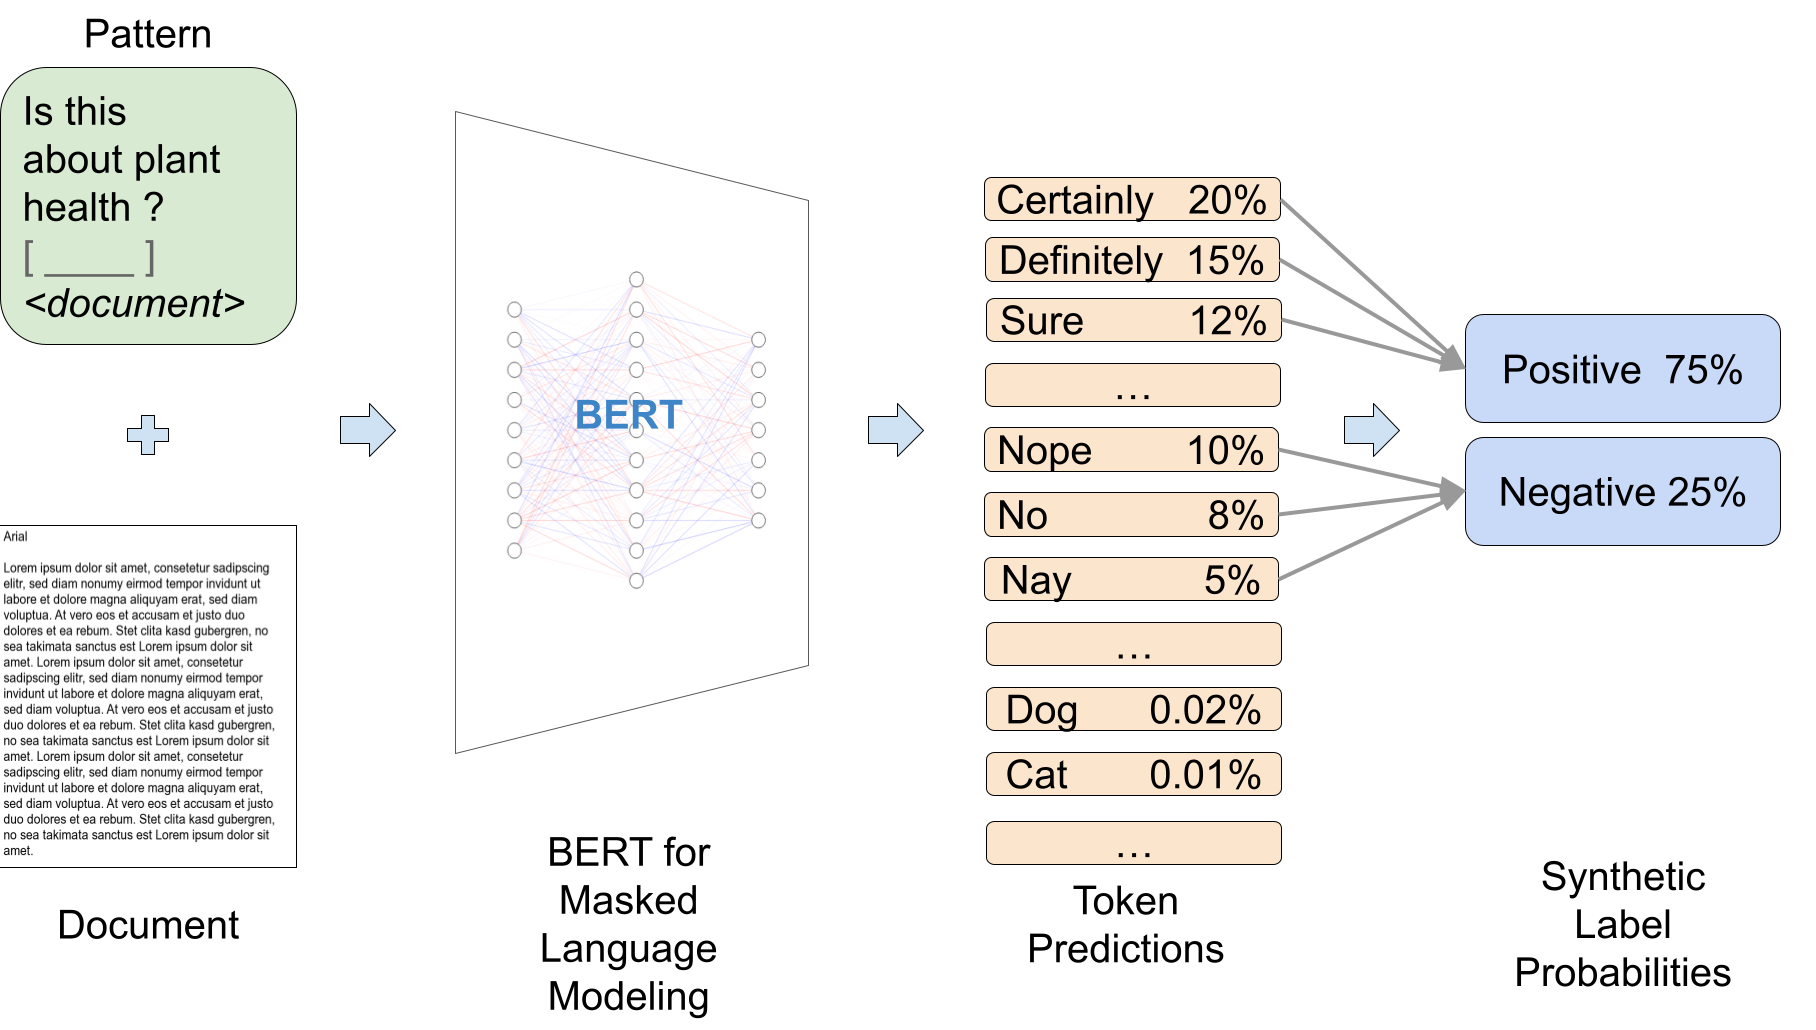
\includegraphics[width=\textwidth]{Figures/06/06_pet_intuition.png}
    \caption{Intuition behind \PET{}}
    \label{fig:06_pet_intuition}
\end{figure}


Implementing \gls{pet} is more intricate. It requires creating multiple patterns, with each pattern aimed at guiding the model's token predictions by emphasizing different aspects of the task. Additionally, each category requires its own verbalizer. It's important to remember that the model's vocabulary is tied to its tokenization method. For instance, in Figure \ref{fig:06_pet_intuition}, while we use terms like ``Definitely", in reality it might be tokenized differently, like ``Definite-ly". We're generally limited to concealing a single token, even though there are ways to expand this\footnote{The \gls{pet} paper's authors suggest a method for multiple tokens, however, the trade-off is that the training time increases significantly}.



In our case, we aim to determine if a document is relevant to Plant Health Surveillance using the \gls{bert} models discussed in \headerName{} \ref{06_bert_models}. 
Each \gls{bert} model has a unique vocabulary and tokenization technique, so we had to pick words that would be consistently tokenized across models. 
As our task is Binary Classification, we opted to create patterns using polar questions\footnote{Polar questions typically have a "yes/no" answer}.
Given the 512-token input limit of \gls{bert} models and the length of some documents, we ensured the masked token was positioned early in the input, avoiding patterns like "$<document>$ $<question>$ [\_\_\_]" or "$<document>$ [\_\_\_] $<question>$".
After initial tests revealed that \gls{pet} training took much longer than \finetuning{}, we settled on just three patterns. The specific patterns and verbalizers we used are detailed in Table \ref{tab:06_pet_patterns_and_verbalizers}.

\begin{table}%[]
    \centering
    \begin{tabular}{l|c}
     \multicolumn{1}{c|}{\textbf{Pattern}} &  \textbf{Verbalizers} \\ \hline
      Is this about plant health? [\_\_\_] $<document>$   & Relevant $\to$ \texttt{yes} \\
      Is this relevant? [\_\_\_] $<document>$   & Irrelevant $\to$ \texttt{no} \\
      Is this about epidemic surveillance? [\_\_\_] $<document>$   & \
    \end{tabular}
    \caption{Patterns and Verbalizers used for \PET{} }
    \label{tab:06_pet_patterns_and_verbalizers}
\end{table}


The \gls{pet} method involves two steps: first training multiple models to generate synthetic labels, followed by fine-tuning a model for classification.

Unlike conventional training approaches, \gls{pet} requires dividing the dataset into \emph{four} distinct splits: training, development, testing, and an additional split of unlabeled documents known as the \emph{unlabeled} split. The rationale behind this will become clear as we delve deeper into the method. Given that this technique is designed for Few-shot learning, the training split typically has only few entries per category.
These probabilities are then combined by averaging their logits for each token\footnote{Meaning, the aggregated logit for a token is the average of the logits generated by the ensemble models.} and using \gls{softmax} to determine a probability for every vocabulary token.
Subsequently, the verbalizers transform the probabilities of pertinent tokens into category label probabilities. 
These synthetic label probabilities are then compared against the true labels in order to calculate a cross entropy loss.
This procedure is depicted in Figure \ref{fig:06_pet_1_pet_ensemble}\footnote{This approach bears some similarity to the "distillation" method introduced by \mytextcite{distilbert}}.


Simultaneously, during this phase, the ensemble models undergo training for \gls{mlm} on our dataset to learn the typical contexts for our task\footnote{We haven't provided a visual representation for this process}. This method of training an ensemble for both synthetic annotation and \gls{mlm} on a dataset requires a custom loss function, which the authors define as a weighted sum of the cross-entropy loss and the \gls{mlm} loss.

% L = L_CE + L_MLM





\begin{figure}
    \centering
    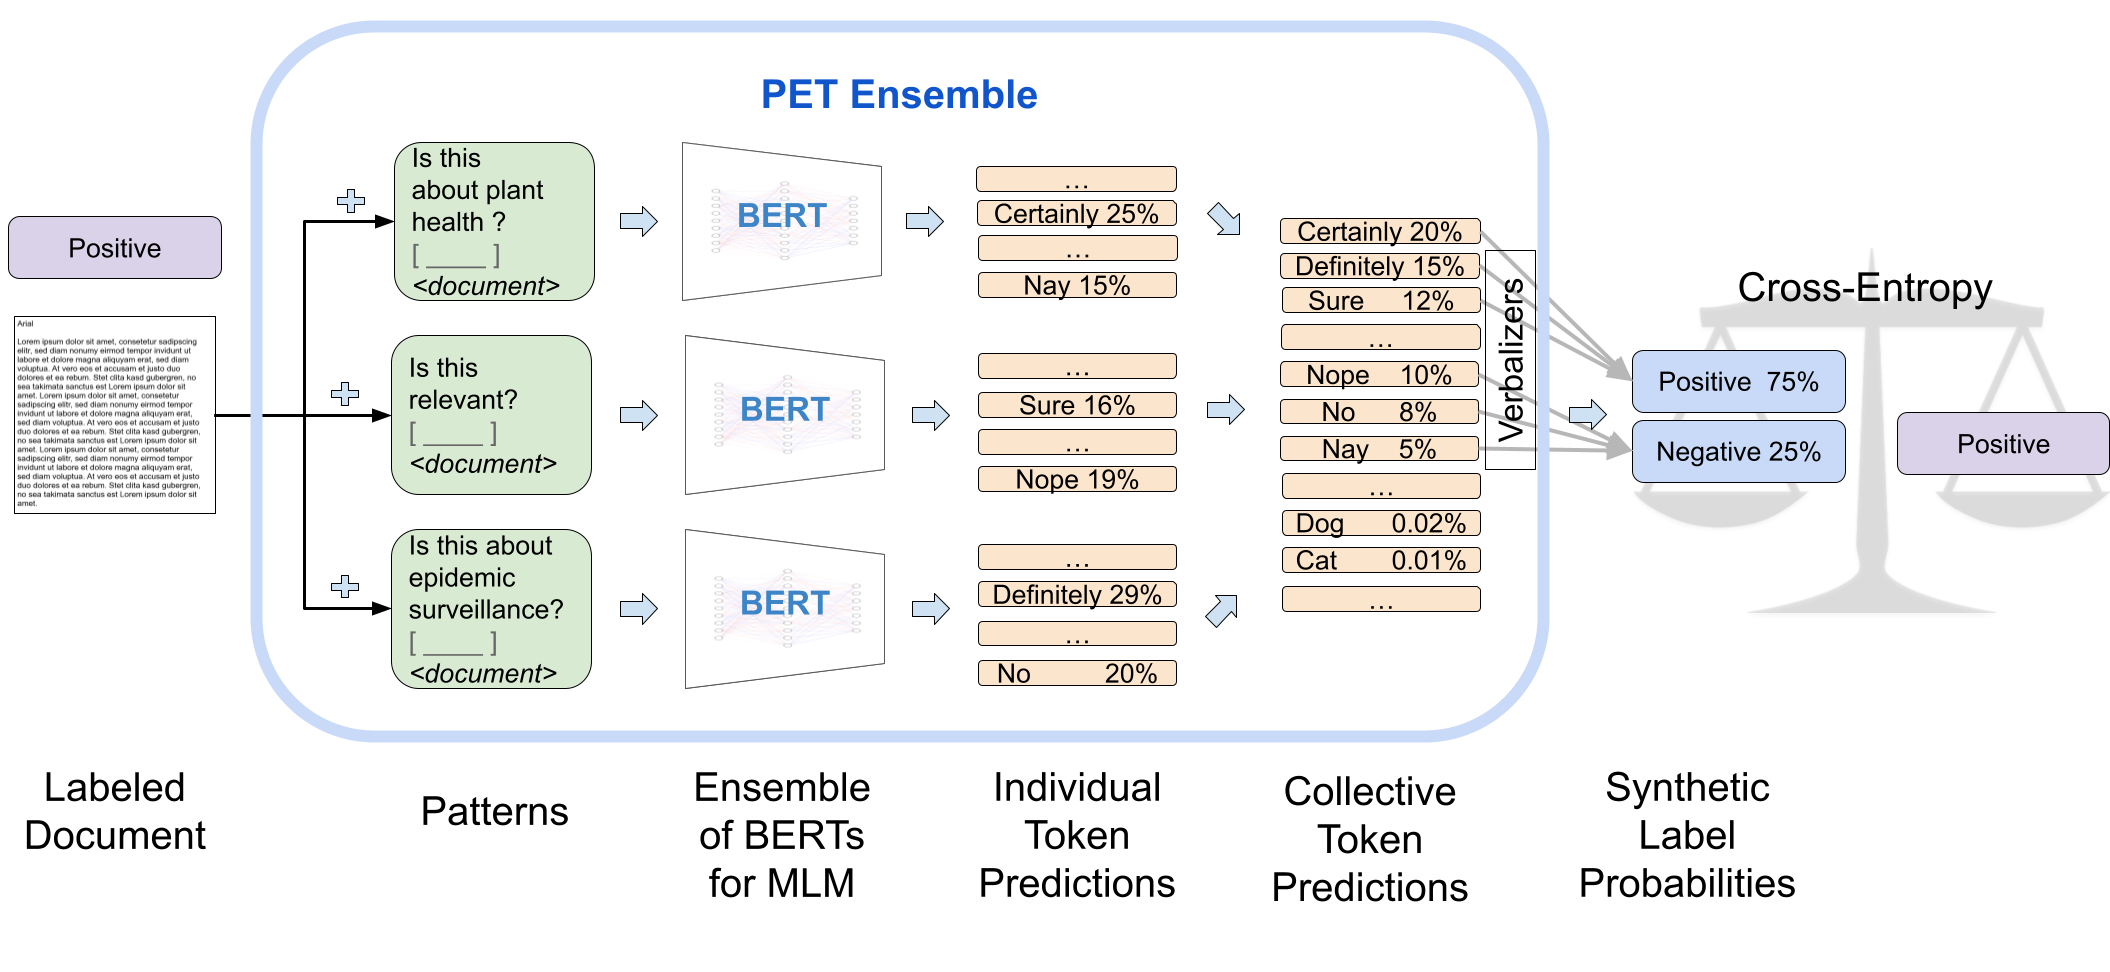
\includegraphics[width=\textwidth]{Figures/06/06_pet_training_1_pet_ensemble.png}
    \caption{Training a \PET{} Ensemble}
    \label{fig:06_pet_1_pet_ensemble}
\end{figure}


The second phase of \gls{pet} involves utilizing the trained \gls{pet} ensemble to generate synthetic labels for the unlabeled documents. 
This synthetically labelled dataset is then employed to fine-tune a new copy of the \gls{bert} model (\bertmultilingual{} in our example) for Document Classification, as detailed in \headerName{} \ref{06_finetuning} above. 
The fine-tuned model, along with its trained classification layer, will act as our Document Classifier (See Figure \ref{fig:06_pet_2_synthetic_finetuning}).

It's worth noting that each phase in \gls{pet} could, in principle, have distinct hyperparameters. Yet, mirroring the original authors' approach, we opted to use the same hyperparameters across both phases for our experiments.

In this work, we opted to utilize \gls{pet} with varying training sizes, including 50, 100, 200, 500, and 1000 documents \emph{per category}.

Next, we detail the method we used to divide the dataset for \finetuning{} and \gls{pet}.


\begin{figure}
    \centering
    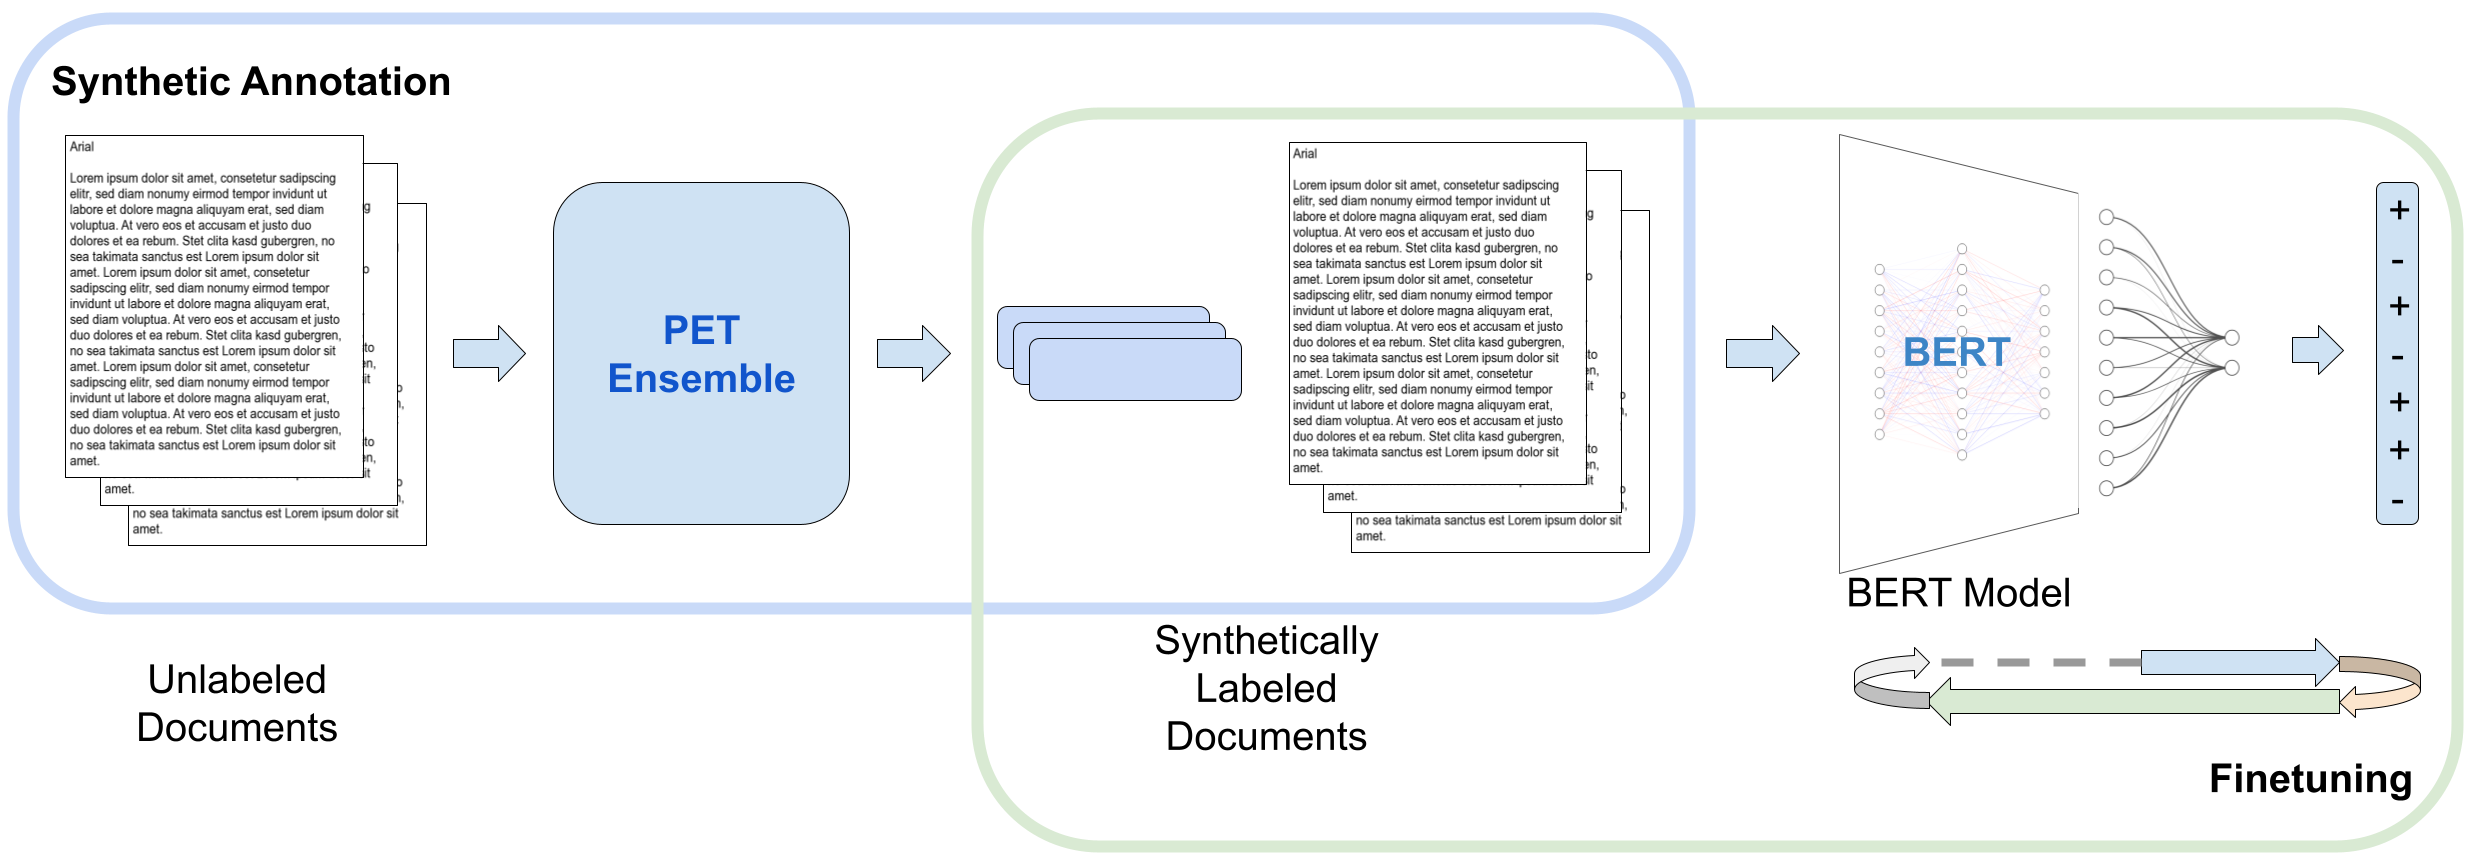
\includegraphics[width=\textwidth]{Figures/06/06_pet_training_2_synthetic_finetuning.png}
    \caption{Creating a Synthetically Labeled Dataset with the \PET{} Ensemble, and subsequently \finetuning{}}
    \label{fig:06_pet_2_synthetic_finetuning}
\end{figure}

